\chapter{Обзор предметной области}
В этой главе описываются основные понятия и термины предметной области, к которой относится представленная работа. Также проводится обзор имеющихся алгоритмических решений и формулируется постановка задачи.

\section{Многокритериальная оптимизация}
Принципиальное отличие многокритериальных задач оптимизации от однокритериальных заключается в том, что во втором случае целью является поиск самого оптимального решения.
В случае же задачи многокритериальной оптимизации такого решения может не существовать вследствие возможных конфликтов значений целевых функций.
Таким образом, многокритериальная оптимизация основывается на компромиссном поиске группы оптимальных решений в смысле Парето.

Большое количество задач, возникающих в различных сферах деятельности человека, представляет собой задачи многокритериальной оптимизации.
В качестве примеров областей применения можно привести оптимальный дизайн и управление в промышленности, моделирование систем, задачи планирования, машинное обучение и анализ данных, биоинформатику, экономику и финансы, управление ресурсами и многое другое.

\section{Основные определения}
\begin{definition}
    В $M$-мерном пространстве, точка $A = (a_1, \ldots, a_M)$ \textit{доминирует в смысле Парето} точку $B = (b_1, \ldots, b_M)$, когда для всех $1 \leq i \leq M$ выполняется неравенство $a_i \leq b_i$ и существует хотя бы одно такое $j$, что $a_j < b_j$.
\end{definition}
\begin{definition}
    Множество оптимальных по Парето недоминируемых решений называется \textit{Парето-фронтом}.
\end{definition}
\begin{definition}
\textit{Недоминирующая сортировка} множества точек $S$ в $M$-мерном пространстве --- это процедура, в процессе которой всем точкам, которые не доминируются никакими другими точками, назначается ранг $0$.
Всем точкам, которые доминируются только точками с рангом $0$, назначается ранг $1$, и т.д.
Все точки с рангом $i$ доминируются только точками с рангом не более $i - 1$.
\end{definition}

\begin{figure}[h]
\centering
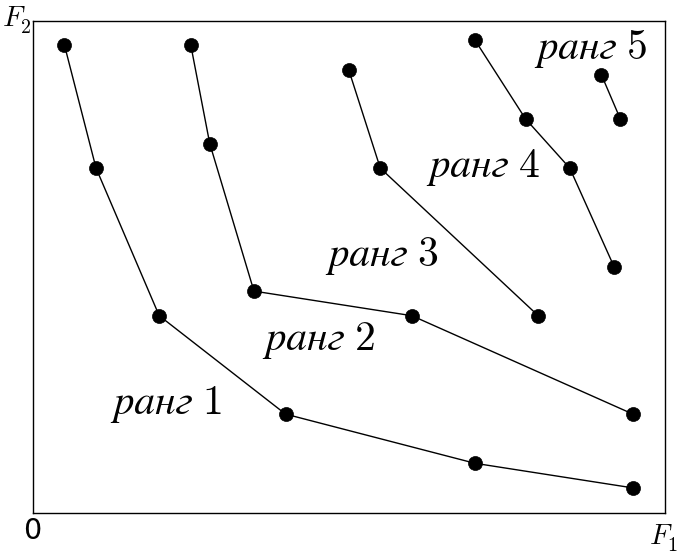
\includegraphics[width=0.7\textwidth]{images/nds.png}
\caption{Недоминирующая сортировка}
\label{pic0}
\end{figure}

\section{Обзор существующих алгоритмов}
\subsection{Наивный алгоритм}
Рассмотрим самую очевидную версию алгоритма недоминирующей сортировки.
Найдем все недоминируемые точки с нулевым рангом, вычеркнем эти точки и будем повторять эту процедуру, каждый раз назначая ранг на единицу больше, чем на предыдущей итерации.
В таком случае, если $M$ --- количество критериев отбора или размерность множества точек (решений), а $N$ --- количество решений, нам необходимо за время $O(MN^2)$ сравнить $O(N^2)$ пар точек по каждому из $M$ критериев и повторить эту процедуру в худшем случае $N$ раз.
Таким образом получаем время работы $O(MN^3)$.

Кунг и др.~\cite{kung75} в своей работе предложили алгоритм поиска оптимальных в смысле Парето решений со сложностью $O(N\log^{M-1}N)$.
Совместив предложенный алгоритм с идеей удаления найденных точек, описанной в наивном алгоритме, мы получаем алгоритм недоминирующей сортировки с общей сложностью $O(N^2\log^{M-1}N)$ в худшем случае, если максимальный ранг решений --- $O(N)$.

\subsection{Быстрая недоминирующая сортировка}
Деб~\cite{deb00} в своей работе предложил алгоритм <<Быстрой недоминирующей сортировки>> в рамках разработки алгоритма NSGA-II, улучшив асимптотическую сложность алгоритма до $O(MN^2)$.
Этот алгоритм является базисным с точки зрения эффективности в семействе алгоритмов, следующим парадигме <<Разделяй и властвуй>>.

Йенсен~\cite{jensen03} был первым, кто предложил алгоритм недоминирующей сортировки со сложностью $O(N\log^{M-1}N)$, позволив тем самым эффективно вычислять ранги точек для типичных конфигураций входных значений.
Однако его алгоритм имел существенный недостаток: он работал корректно только в предположении, что никакие два решения не имеют одинаковых значений по одному и тому же критерию.

Фанг и др.~\cite{fang08} в своей работе пришли к заключению, что алгоритм Йенсена не способен воспроизводить такие же недоминирующие фронты точек, как оригинальный алгоритм NSGA-II.
Исследователи продемонстрировали, что устранение главного недостатка алгоритма Йенсена является нетривиальной задачей, так как существует множество крайних случаев, требующих отдельного рассмотрения.

Решение данной проблемы было предложено Фортеном и др.~\cite{fortin13}.
Предложенный им <<обобщенный>> алгоритм недоминирующей сортировки работает корректно на любых входных данных, сохраняя при этом среднюю временную сложность $O(N\log^{M-1}N)$.
Тем не менее было доказано, что в худшем случае время работы алгоритма составляет $O(N^2M)$.

Дальнейшее улучшение недоминирующей сортировки Фортена было предложено Буздаловым и Шалыто~\cite{buzdalov14}.
В своей работе они модифицируют алгоритм и доказывают оценку $O(N\log^{M-1}N)$ для худшего случая.
Более подробное описание алгоритма с модификацией будет представлено ниже.

\subsection{Алгоритм Роя}
В одной из недавних публикаций Рой и др.~\cite{roy16} предложили алгоритм <<Best Order Sort>> с вычислительной сложностью $O(MN\log{M}+MN^2)$.
В основе алгоритма лежит следующая идея: для каждой точки $p$ по каждому из $M$ критериев можно составить множество точек, доминируемых точкой $p$.
Соответственно, для определения ранга точки $p$ достаточно рассмотреть только одно из этих множеств.

Основной целью алгоритма является уменьшение количества сравнений.
В худшем случае время его работы --- $O(MN^2)$, но на некоторых входных данных алгоритм может работать за $O(MN\log{M})$.
Авторы не предоставляют более строгого теоретического исследования эффективности данного алгоритма.
Как показывает практика, алгоритм демонстрирует не самые лучшие результаты при больших размерах входных данных.
В рамках представленной работы данный алгоритм интереса не представляет.

\section{Описание алгоритма <<Разделяй и властвуй>>}
Алгоритм Фортена состоит из нескольких процедур:
\begin{itemize}
    \item $NonDominatedSort(S, K)$ --- процедура недоминирующей сортировки, получающая на вход множество точек $S$ и размерность $K$ и возвращающая результат недоминирующей сортировки --- последовательность Парето-фронтов, содержащих точки исходного множества.
Внутри процедуры осуществляется лексикографическая сортировка входящих точек, всем точкам назначается нулевой ранг и вызывается процедура $NDHelperA$.
    \item $NDHelperA(S, k)$ --- основная процедура алгоритма. В ней вычисляются ранги точек множества $S$ на основывании первых $k$ критериев. Псевдокод представлен в листинге.
    \item $NDHelperB(L, H, k)$ назначает ранги точкам из множества $H$, сравнивая их с точками из множества $L$, основываясь на первых $k$ критериях. Псевдокод также представлен в листинге.
    \item $SweepA(S)$ --- это процедура, определяющая ранги точек по первым двум координатам, используя метод заметающей прямой. Время ее работы --- $O(|S|\log|S|)$.
    \item $SweepB(L, H)$ определяет ранги точек из множества $H$, сравнивая их с точками множества $L$ по первым двум критериям. В ней также используется метод заметающей прямой, а время ее работы --- $O((|L| + |H|)\log{|L|})$.
    \item $SplitA(S, k)$ разделяет множество точек $S$ на два подмножества, сравнивая $k$-ю координату каждой точки с медианным значением. Точки, имеющие по $k$-му критерию значение, равное медиане, добавляются к меньшему из двух подмножеств.
    \item $SplitB(L, H, k)$ разделяет каждое из множеств $L$ и $H$ на два, используя аналогичную процедуру. В качестве опорного элемента используется медиана $k$-х координат большего из двух исходных множеств.
\end{itemize}

Стоит отметить, что все вышеперечисленные процедуры сохраняют лексикографический порядок исходных множеств.
Это условие позволяет утверждать, что точка $A$, лежащая во входном списке правее точки $B$, никогда не будет доминировать точку $B$.

Буздалов и Шалыто предложили модифицировать процедуры $SplitA$ и $SplitB$, а также соответственно вызывающие их процедуры $NDHelperA$ и $NDHelperB$. Вместо первых двух будет использоваться метод $SplitBy(S, m, k)$, который разделяет входящее множество точек $S$ не на две, а на три части:
\begin{itemize}
    \item $L$ --- множество точек, $k$-я координата которых меньше $m$;
    \item $M$ --- множество точек, $k$-я координата которых равна $m$;
    \item $H$ --- множество точек, $k$-я координата которых больше $m$;
\end{itemize}

\begin{algorithm}[!h]
\caption{Процедура SplitBy. Разделение точек из $S$ на три подмножества по $k$-му критерию относительно значения $m$.}\label{lst0}
\begin{algorithmic}
\Procedure{SplitBy}{S, m, k}
    \State $L \gets \{s \in S\mid s_k < m\}$
    \State $M \gets \{s \in S\mid s_k = m\}$
    \State $H \gets \{s \in S\mid s_k > m\}$
\EndProcedure
\end{algorithmic}
\end{algorithm}

\begin{algorithm}[!h]
\caption{Процедура NDHelperA. Определение рангов точек из $S$ по $k$ первым критериям.}\label{lst1}
\begin{algorithmic}
\Procedure{NDHelperA}{S, k}
    \If{$|S| < 2$}
        \State \Return
    \ElsIf{$|S| = 2$}
        \State $\{s^{(1)}, s^{(2)}\}\gets S$
        \If{$s_{1:k}^{(1)} \prec s_{1:k}^{(2)}$}
            \State $RANK(S^{(2)})\gets \max\{RANK(S^{(2)}), RANK(S^{(1)})+1\}$ 
        \EndIf
    \ElsIf{$k = 2$}
        \State$\textsc{SweepA}(S)$
    \ElsIf{$|\{s_k \mid s \in S\}| = 1$}
        \State $\textsc{NDHelperA}(S, k-1)$
    \Else
        \State $L,M,H \gets \textsc{SplitBy}(S, median\{s_k\mid s \in S\}, k)$
        \State $\textsc{NDHelperA}(L, k)$
        \State $\textsc{NDHelperB}(L, M, k-1)$
        \State $\textsc{NDHelperA}(M, k-1)$
        \State $\textsc{NDHelperB}(L \cup M, H, k-1)$
        \State $\textsc{NDHelperA}(H, k)$
    \EndIf
\EndProcedure
\end{algorithmic}
\end{algorithm}

\begin{algorithm}[!h]
\caption{Процедура NDHelperB. Назначение рангов точкам из $H$ относительно точек из $L$ по $k$ первым критериям.}\label{lst2}
\begin{algorithmic}
\Procedure{NDHelperB}{L, H, k}
    \If{$|L| = 0$ or $|H| = 0$}
        \State \Return
    \ElsIf{$|L| = 1$ or $|H| = 1$}
        \ForAll{$h \in H, l \in L$}
            \If{$l_{1:k} \preceq h_{1:k}$}
                \State $RANK(h) \gets \max\{RANK(h), RANK(l) + 1\}$
            \EndIf
        \EndFor
    \ElsIf{$k = 2$}
        \State $\textsc{SweepB}(L, H)$
    \ElsIf{$ \max\{l_k\mid l \in L\} \leq \min\{h_k\mid h \in H\}$}
        \State $\textsc{NDHelperB}(L, H, k-1)$
    \Else
        \State $m \gets median\{s_k\mid s \in L \cup H\}$
        \State $L_1, M_1, H_1 \gets \textsc{SplitBy}(L, m, k)$
        \State $L_2, M_2, H_2 \gets \textsc{SplitBy}(H, m, k)$
        \State $\textsc{NDHelperB}(L_1, L_2, k)$
        \State $\textsc{NDHelperB}(L_1, M_2, k-1)$
        \State $\textsc{NDHelperB}(M_1, M_2, k-1)$
        \State $\textsc{NDHelperB}(L_1 \cup M_1, H_2, k-1)$
        \State $\textsc{NDHelperB}(H_1, H_2, k)$
    \EndIf
\EndProcedure
\end{algorithmic}
\end{algorithm}


\section{Существующие параллельные алгоритмы}
\subsection{Параллельный NSGA-II}
В своей работе Гупта и Тэн~\cite{gupta15} представили хорошо масштабируемую реализацию алгоритма недоминирующей сортировки, заточеную под многоядерные графические процессоры.
Однако их разработка имеет некоторые недостатки. В качестве базового алгоритма исследователи использовали стандартную реализацию NSGA-II с квадратичным временем работы.
Несмотря на хорошую масштабируемость, алгоритм сильно проигрывает по общему объему работы, производя большое количество лишних вычислений.
Существенный прирост в производительности в их разработке достигается только при очень большом количестве процессоров. 
Исследователи продемонстрировали ускорение в $4.5$ --- $10.6$ раз относительно оригинальной версии NSGA-II на графическом процессоре со 192 ядрами.
В данной статье будет произведено сравнение эффективности данного алгоритма с предлагаемым нами решением.

\subsection{Параллельная сортировка слиянием}
Мишра и др.~\cite{mishra16} предложили свою версию недоминирующей сортировки, напоминающую сортировку слиянием.
Предложенный алгоритм состоит из двух фаз: лексикографической сортировки решений и непосредственного вычисления рангов.
Во второй фазе каждой точке назначается ранг $1\leq i \leq N$ и создаются множества Парето-фронтов, которые впоследствии будут cливаться воедино, пока ранги не будут вычислены.
Авторы замечают, что слияние пар Парето-фронтов на каждом уровне может производиться независимо друг от друга, и делают предположение о возможности параллельного исполнения алгоритма.
Теоретического обоснования или подробного экспериментального исследования эффективности параллельного алгоритма в работе не представлено.

\section{Постановка задачи}
Как было сказано ранее, разработка быстрых алгоритмов недоминирующей сортировки крайне важна для эффективного решения задач многокритериальной оптимизации и поэтому является актуальной задачей.

Алгоритм Фортена в модификации Буздалова обладает оптимальным теоретическим временем работы и показывает хорошие результаты на больших объемах входных данных.
Тем не менее, этот алгоритм не использует возможностей многопроцессорных систем, в связи с чем возникает задача его модификации для параллельного исполнения.
